\section{Introducción}
A lo largo de este capítulo se analiza un ejemplo de aplicación.
Dicho caso sirve para demostrar las funcionalidades que ofrece \nombreFramework
\ Framework. El mismo consiste en un sistema de clasificación y lavado de
botellas.

\section {Sistema de Clasificación y Lavado de Botellas}
A continuación se describen las características principales de un sistema de
lavado de botellas:

\begin{itemize}
  \item El ingreso de botellas no es controlado por el sistema.
  \item Las botellas pueden ser depositadas en la máquina en cualquier instante
  de tiempo de forma asincrónica para el sistema.
  \item La clasificación de las botellas se realiza en un módulo que
  diferencia entre \emph{cerveza}, \emph{gaseosa} u \emph{otras}.
  \item Puede haber un máximo de 20 botellas en la etapa de
  recepción y clasificación.
  \item La recepción de botellas tiene máxima prioridad siempre que pueda
  realizarse.
  \item Puede iniciarse la recepción de una botella antes de finalizar
  la recepción de la botella anterior.
  \item Mientras la máquina se encuentra en proceso de clasificación de
  botellas, no puede iniciar la recepción de una nueva botella.
  \item Cuando la máquina no puede recibir una botella, la misma queda en espera
  para ser procesada.
  \item El proceso completo de lavado para una botella de gaseosa consta de los
  siguientes pasos:
      \begin{itemize} 
        \item Lavado con agua a presión.
        \item Secado.
      \end{itemize}
  \item El proceso completo de lavado para una botella de cerveza consta de los
  siguientes pasos:
      \begin{itemize} 
        \item Lavado con agua a presión y detergente.
        \item Enjuague.
        \item Secado.
      \end{itemize}
  \item Si se inserta una botella de otro tipo, la misma es expulsada de la
    máquina sin lavar.
  \item La máquina sólo puede procesar una botella por vez en cada uno de sus
  módulos.
  \item Al finalizar el proceso de lavado las botellas son devueltas por la
  máquina, utilizando una salida independiente de la entrada.
  
\end{itemize}

\begin{figure}[H]
    \centering
    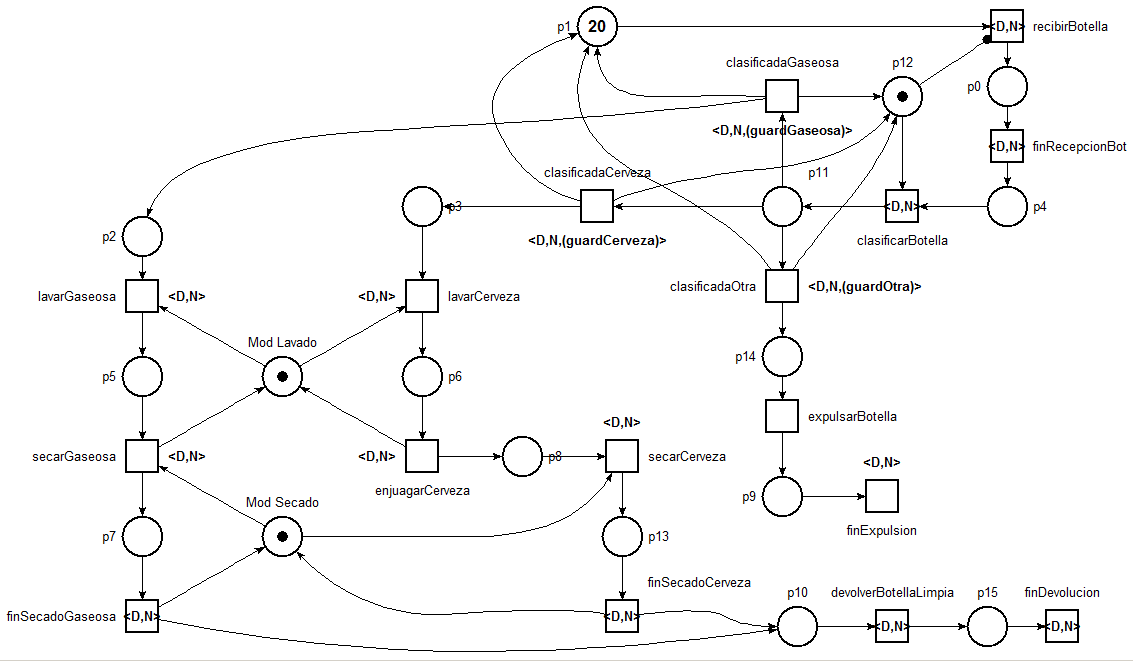
\includegraphics[width=120mm]{petri_lavadora_botellas}
    \caption{Modelo en Red de Petri de la Lógica de un Sistema de Clasificación y
    Lavado de Botellas}
    \label{fig:petri_lavadora_botellas}
\end{figure}

\subsection {Pasos para el desarrollo del sistema utilizando  \\
\nombreFramework \  Framework}
\label{sec:pasos_desarrollo_lavadora_botellas}
Tras el modelado de la lógica del sistema en la Red de Petri, el
proceso de desarrollo del sistema puede descomponerse en una serie de
pasos a resolver.
De esta manera se comprende fácilmente el proceso para crear un sistema
utilizando el framework.

\begin{enumerate}
\item \textbf{Determinar los objetos para conformar el sistema:}\\
        Como en cualquier desarrollo orientado a objetos, uno de los pasos principales
        del diseño es la identificación de los objetos que intervienen en el sistema,
        para luego obtener las clases.
        En este caso se identifican los siguientes:
            \begin{itemize}
              \item Botellas insertadas.
              \item Máquina lavadora compuesta por:
              \begin{itemize}
                  \item Módulo de clasificación de botellas.
                  \item Módulo de lavado.
                  \item Módulo de enjuague.
                  \item Módulo de secado.
                  \item Módulo de expulsión de botellas incorrectas.
                  \item Colas donde se almacenan las botellas durante el proceso.
              \end{itemize}
            \end{itemize}

\item \textbf{Determinar las acciones de los objetos del sistema:}\\
            Otro paso principal en el desarrollo orientado a objetos es determinar las
            acciones que pueden realizar los objetos del sistema. Estas acciones serán
            embebidas en los métodos controladores de acciones de las clases
            desarrolladas.
            En este caso, las acciones son realizadas por la máquina lavadora, y se
            identifican las siguientes:
            \begin{itemize}
              \item Recibir botellas.
              \item Clasificar botellas.
              \item Lavar botellas de gaseosa.
              \item Secar botellas de gaseosa.
              \item Lavar botellas de cerveza.
              \item Enjuagar botellas de cerveza.
              \item Secar botellas de cerveza.
              \item Expulsar botellas incorrectas.
              \item Devolver botellas limpias.
            \end{itemize}

\item \textbf{Clasificar Happening Controllers y Task Controllers:}\\
            Los controladores de acciones pueden procesar eventos físicos de entrada
            (Eventos Happening) o emitir eventos físicos de salida (Eventos Task). Es
            importante determinar a cuál grupo pertenece cada acción del
            sistema, para poder clasificarla como Happening Controller o Task Controller (ver
            sección~\ref{sec:controladores_de_acciones}).
            Esta clasificación se realiza en el software a través de las anotaciones Java
            @HappeningController y @TaskController. En el caso de ejemplo se distinguen:
            \begin{itemize}
              \item Happening Controllers:
                  \begin{itemize}
                    \item Recibir botellas.
                  \end{itemize}
              \item Task Controllers:
                  \begin{itemize}
                  \item Clasificar botellas.
                  \item Lavar botellas de gaseosa.
                  \item Secar botellas de gaseosa.
                  \item Lavar botellas de cerveza.
                  \item Enjuagar botellas de cerveza.
                  \item Secar botellas de cerveza.
                  \item Expulsar botellas incorrectas.
                  \item Devolver botellas limpias.
                  \end{itemize}
            \end{itemize}

\item \textbf{Manejo de guardas:}\\
            En determinadas ocasiones, es necesario representar
            estados externos que no están modelados en la red. Para lograr esto asociamos
            una variable booleana que representa el estado externo a una transición.
            Actuando la misma como un factor de sensibilización externo (ver
            secciónes~\ref{sec:guardas_monitor} y \ref{guardas}).
            Para alterar el valor de una guarda, debe definirse un método del tipo Guard Provider
            asociado a dicha guarda, utilizando la anotación Java @GuardProvider en el
            código del software (ver sección~\ref{sec:guard_providers}).
    
\item \textbf{Definir la prioridad de las acciones:}\\
            A veces es necesario definir prioridades específicas para la ejecución de los
            controladores de acciones. Estas prioridades se manejan a través del monitor
            de redes de Petri, mediante la utilización de políticas de disparo de
            transición. El usuario puede utilizar las políticas proporcionadas por el
            framework (transición aleatoria o primera transición en línea) o definir una
            política a su medida como se explica en la sección~\ref{sec:politica_transiciones}.
            De acuerdo a las características descriptas para este caso, la transición
            ``recibirBotella'' debe tener máxima prioridad.

\item \textbf{Definir la cantidad de Hilos de ejecución:}\\
            Si bien no existe una respuesta absoluta, en términos generales se busca
            optimizar la performance minimizando la cantidad de hilos de ejecución
            posibles sin afectar al paralelismo del programa. Para lo cual se determinan
            aquellos Task Controllers secuenciales, que sólo requieren un único hilo para
            su ejecución, y se los agrupa en Complex Secuential Task Controllers (ver
            sección~\ref{sec:complex_secuential_task_controller}).
            Se distinguen los siguientes hilos de ejecución, donde se especifica quién
            está a cargo de la creación e inicialización del hilo (el control de la
            ejecución lo realiza el monitor en todos los casos):
            \begin{itemize}
              \item \textbf{Happening Controllers \emph{(A cargo del usuario)}:}
                  \begin{enumerate}[label=\fbox{\arabic*}]
                    \item Recibir botellas. 
                  \end{enumerate}
              \item \textbf{Task Controllers \emph{(A cargo del framework)}:}
                  \begin{enumerate}[resume , label=\fbox{\arabic*}]
                  \item Clasificar botellas.
                  \item Expulsar botellas incorrectas.
                  \item Devolver botellas limpias.
                  \end{enumerate}
              \item \textbf{Complex Secuential Task Controllers \emph{(A cargo
              del framework)}:} \begin{enumerate}[resume, label=\fbox{\arabic*}]
                    \item Proceso de lavado de botellas de gaseosa.
                        \begin{itemize}
                          \item Lavar botellas de gaseosa.
                          \item Secar botellas de gaseosa.
                      \end{itemize}
                    \item Proceso de lavado de botellas de cerveza.
                        \begin{itemize}
                          \item Lavar botellas de cerveza.
                          \item Enjuagar botellas de cerveza.
                          \item Secar botellas de cerveza.
                      \end{itemize}
                  \end{enumerate}
            \end{itemize}

\item \textbf{Determinar la relación entre la Red de Petri, los métodos y las clases:}\\
            La ejecución de los controladores de acciones está relacionada con el
            disparo de las transiciónes en la Red de Petri. Por eso, es necesario 
            relacionar dichas transiciones con los objetos y métodos correspondientes.
            Dicha tarea se realiza a través de un archivo JSON, configurable por el
            usuario, donde se definen los tópicos (ver
            sección~\ref{sec:relacion_evento_controlador}). Tras crear el archivo, el
            usuario debe suscribir cada objeto y método que sean parte de un controlador
            de acción a un tópico. Esta suscripción se realiza en el código del software.
\end{enumerate}

\subsection {Implementación del sistema utilizando \nombreFramework}

En esta sección se analiza una implementación del sistema de
lavado y clasificación de botellas. En esta implementación en particular, el
mundo físico externo al sistema es representado por una Interfaz Gráfica de
Usuario. 

En la figura~\ref{fig:diagrama_clases_lavadora_botellas} se observa el diagrama
de clases del sistema. El usuario es el encargado de definir las interfaces y
herencias que considere necesarias para implementar las funcionalidades del
sistema.
\begin{figure}[H]
    \centering
    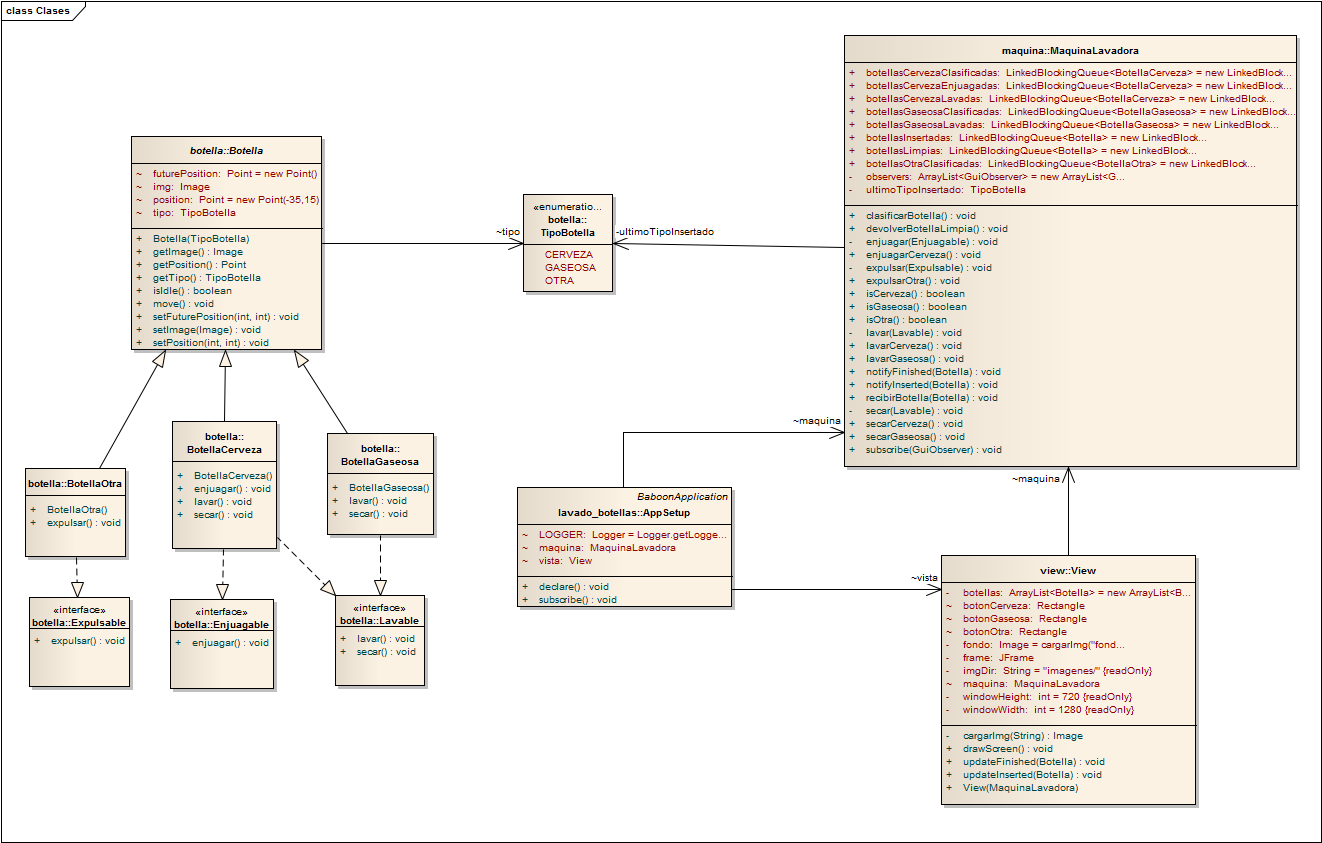
\includegraphics[width=120mm]{diagrama_clases_lavadora_botellas}
    \caption{Diagrama de Clases de un Sistema de Clasificación y Lavado de
    Botellas.}
    \label{fig:diagrama_clases_lavadora_botellas}
\end{figure}

Aquellos métodos que forman parte de un controlador de acción deben
clasificarse y etiquetarse en el código con \emph{@HappeningController} o
\emph{@TaskController}. Por ejemplo:\\

\begin{minted}{java}
  @TaskController
  public void lavarGaseosa(){
    BotellaGaseosa botella = botellasGaseosaClasificadas.poll();
    lavar(botella);
    botellasGaseosaLavadas.add(botella);
  }
\end{minted}

\begin{minted}{java}
  @HappeningController
  public void recibirBotella(Botella botella){
    botellasInsertadas.add(botella);
  }
\end{minted}

El manejo de las guardas se realiza mediante la definición de métodos anotados
con \emph{@GuardProvider}. Por ejemplo:\\

\begin{minted}{java}
  @GuardProvider("guardCerveza")
  public boolean isCerveza(){
    return ultimoTipoInsertado.equals(TipoBotella.CERVEZA);
  }
\end{minted}

El manejo de prioridades se realiza mediante la implementación de una política
de disparo de transiciones personalizada. En la definición de las
características del problema se estableció que la transición ``recibirBotella''
debe tener máxima prioridad. Para ello se creó una clase
\emph{InsertBottlesFirstPolicy} que hereda de \emph{TransitionsPolicy} e
implementa el método \emph{which()}. 

\begin{framed}
\textbf{Nota:} El usuario no debe instanciar un objeto de la clase
\emph{InsertBottlesFirstPolicy}. Al momento de crear el monitor de petri se
indica cuál es la clase que implementa la política de disparos, y el framework
se encarga luego de generar la instancia que será utilizada. De esta forma el
usuario no tiene acceso directo a la RdP desde el código, previniendo
modificaciones indeseadas del estado de la red.
\end{framed}


\begin{minted}{java}

public class InsertBottlesFirstPolicy extends TransitionsPolicy{

  private final int priorityIndex;

  public InsertBottlesFirstPolicy(PetriNet _petri) { 
    super(_petri); 
    priorityIndex = this.petri.getTransition("recibirBotella").getIndex(); 
  }
  
  @Override
  public int which(boolean[] enabled) {
    if(enabled[priorityIndex]){ //Si recibirBotella está habilitada.
      return priorityIndex; //retornar el indice de recibirBotella.
    }
    else {
      //Sino, disparar la primer transición 
      //habilitada que encuentre.
      for(int i = 0; i < enabled.length; i++){
        if(enabled[i]){
          return i; 
        }
      }
    }
    return -1;
  }
}
\end{minted}

En la sección~\ref{sec:pasos_desarrollo_lavadora_botellas} se determinaron 6
hilos de ejecución. Cada uno de los hilos corresponde a un controlador de
acción. A su vez, cada controlador de acción debe suscribirse a
un tópico, por lo que es necesario definir en primer lugar dichos tópicos. Los
mismos se definen a través de un archivo JSON, de la siguiente forma:\\
\begin{minted}{json}
[
  {
    "name" : "recepcion_botella",
    "permission": ["recibirBotella"],
    "fireCallback": ["finRecepcionBot"]
  },
  {
    "name" : "clasificacion_botella",
    "permission": ["clasificarBotella"],
    "fireCallback": ["clasificadaGaseosa", "clasificadaCerveza", "clasificadaOtra"],
    "setGuardCallback" : [["guardCerveza","guardGaseosa","guardOtra"]]
  },
  {
    "name" : "lavado_cerveza",
    "permission" : ["lavarCerveza","enjuagarCerveza","secarCerveza"],
    "fireCallback": ["finSecadoCerveza"]
  },
  {
    "name": "lavado_gaseosa",
    "permission" : ["lavarGaseosa","secarGaseosa"],
    "fireCallback" : ["finSecadoGaseosa"]
  },
  {
    "name" : "expulsion_otra",
    "permission": ["expulsarBotella"],
    "fireCallback" : ["finExpulsion"]
  },
  {
    "name" : "devolucion_botella",
    "permission": ["devolverBotellaLimpia"],
    "fireCallback" : ["finDevolucion"]
  }
]
\end{minted}

Un tópico está relacionado con los eventos lógicos de
disparo de transiciones y de modificación de valor de guardas. Dicha relación
se determina a través del nombre de dichos componentes de la RdP, como
puede apreciarse en la figura~\ref{fig:topic_petri_relacion}.

\begin{figure}[H]
    \centering
    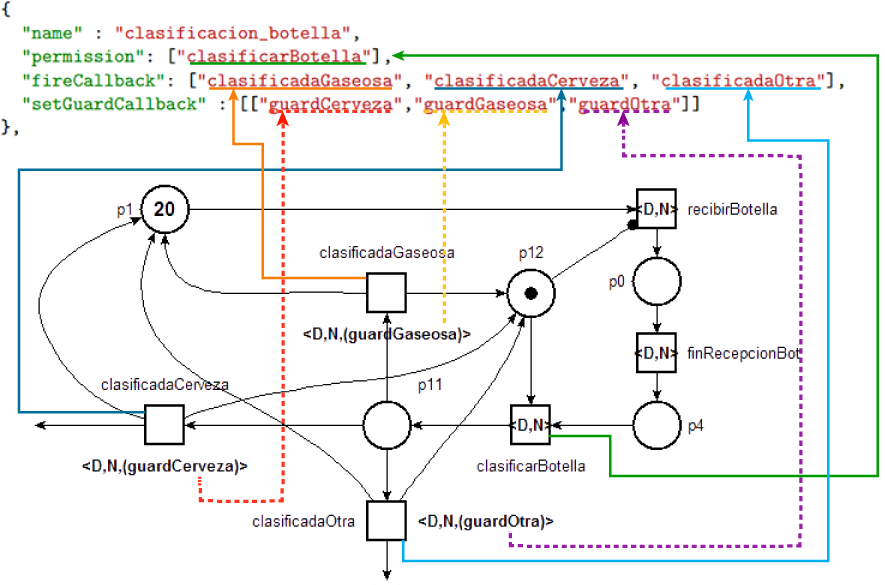
\includegraphics[width=120mm]{topic_petri_relacion}
    \caption{Relación entre un tópico y los componentes de la Red de Petri.}
    \label{fig:topic_petri_relacion}
\end{figure}

Otro aspecto que el usuario debe tener en cuenta, es la
creación e inicialización de los hilos que se encargan de ejecutar los
HappeningController. Esto es responsabilidad del código de usuario. Por
ejemplo, cuando el EventListener que escucha eventos del mouse en la GUI
detecta un evento, se crea un nuevo hilo que ejecuta el HappeningController
encargado de manejar dicho evento (\emph{recibirBotella()}). A
continuación se observa el código descripto:

\begin{minted}{java}
    @Override
    public void mouseClicked(MouseEvent arg0) {
      new Thread( () -> {
        if(botonCerveza.contains(arg0.getPoint())){
          maquina.recibirBotella(new BotellaCerveza());
        }
        else if(botonGaseosa.contains(arg0.getPoint())){
          maquina.recibirBotella(new BotellaGaseosa());
        }
        else if(botonOtra.contains(arg0.getPoint())){
          maquina.recibirBotella(new BotellaOtra());
        }
      }).start();
    }
\end{minted}


Finalmente, se define la clase \emph{AppSetup}, que implementa la interfaz
\emph{BaboonApplication} (ver sección~\ref{sec:componentes_baboon}), donde se
realizan las siguientes actividades:
\begin{itemize}
  \item Inicializar el monitor de RdP con el archivo PNML y la política de
  disparos.
  \item Añadir el archivo de tópicos para configurar los eventos de acción en
  el sistema.
  \item Declarar e inicializar los objetos del sistema.
  \item Suscribir los controladores de acción a los tópicos.
\end{itemize} 

A continuación se observa la implementación de dicha clase con
las actividades descriptas previamente:

\begin{minted}{java}
public class AppSetup implements BaboonApplication {
  private static Logger LOGGER = Logger.getLogger(AppSetup.class.getName());
  private MaquinaLavadora maquina;
  private View vista;

  @Override
  public void declare() {
    //Inicialización de los objetos del sistema
    maquina = new MaquinaLavadora();
    vista = new View(maquina);
    try {
      //Inicialización del core de petri.
      //Notar que se requiere el objeto Class de la política.
      BaboonFramework.createPetriCore("pnml/lavadoBotellas_v2.pnml",
          petriNetType.PLACE_TRANSITION, InsertBottlesFirstPolicy.class);
    } 
    catch (BadPolicyException e) {
      LOGGER.log(Level.SEVERE, "Error configurando la política de disparos.
                     La aplicación terminará ahora.", e);
      System.exit(1);
    }
    try {
      //Inicialización de los tópicos.
      BaboonFramework.addTopicsFile("topic/topics.json");
    } 
    catch (BadTopicsJsonFormat | NoTopicsJsonFileException e) {
      LOGGER.log(Level.SEVERE, "Error inicializando Baboon Framework.
                     La aplicación terminará ahora.", e);
      System.exit(1);
    }

    //Inicialización de thread de GUI
    new Thread( () -> {
      while(true){
        vista.drawScreen();
        try {
          Thread.sleep(25);
        } catch (InterruptedException e) {
           LOGGER.log(Level.INFO, "InterruptedException en thread de GUI", e);
        }
      }
    }).start();
  }

\end{minted}

\begin{minted}{java}
  @Override
  public void subscribe() {
    try {
      //Suscripción de un HappeningHandler.
      //Notar que se usa un objeto BotellaCerveza como parámetro.
      //El framework lo utiliza para determinar el método correcto a
      //utilizar como controlador de acción
      // En este caso, cualquier objeto que herede de
      //la clase abstracta Botella puede ser utilizado.
      BaboonFramework.subscribeControllerToTopic("recepcion_botella", maquina,
          "recibirBotella", new BotellaCerveza());

      //Suscripción de TaskControllers Simples
      BaboonFramework.subscribeControllerToTopic("clasificacion_botella", 
            maquina, "clasificarBotella");
      BaboonFramework.subscribeControllerToTopic("expulsion_otra", 
            maquina, "expulsarOtra");
      BaboonFramework.subscribeControllerToTopic("devolucion_botella", 
            maquina, "devolverBotellaLimpia");

      //Creación de ComplexSecuentialTaskControllers
      BaboonFramework.createNewComplexTaskController("lavarCerveza", "lavado_cerveza");
      BaboonFramework.createNewComplexTaskController("lavarGaseosa", "lavado_gaseosa");

      //Suscripción de TaskControllers a ComplexSecuentialTaskControllers
      BaboonFramework.appendControllerToComplexTaskController("lavarCerveza", 
            maquina, "lavarCerveza");
      BaboonFramework.appendControllerToComplexTaskController("lavarCerveza", 
            maquina, "enjuagarCerveza");
      BaboonFramework.appendControllerToComplexTaskController("lavarCerveza", 
            maquina, "secarCerveza");
      BaboonFramework.appendControllerToComplexTaskController("lavarGaseosa", 
            maquina, "lavarGaseosa");
      BaboonFramework.appendControllerToComplexTaskController("lavarGaseosa",
            maquina, "secarGaseosa");

    } catch (NotSubscribableException e) {
      LOGGER.log(Level.SEVERE, "Error suscribiendo acciones a Baboon Framework.
        La aplicación terminará ahora.", e);
      System.exit(1);
    }
  }
}
\end{minted}

\subsection {Configuración del Entorno de Desarrollo de \nombreFramework
Framework}

La configuración del entorno de desarrollo para \nombreFramework
Framework consta de los siguientes pasos:

\begin{enumerate}
    \item Descargar e instalar Java JDK version \textgreater= 8
    \item Descargar e instalar Eclipse IDE 
    \item Instalar M2Eclipse (Maven):
        \begin{itemize}
            \item En Eclipse, ir a Help -\textgreater Install New Software
        \item Colocar la dirección del repositorio de m2e en el recuadro “Work
              with”.
        \end{itemize}
    \item Instalar AspectJ:
        \begin{itemize}
            \item En Eclipse, ir a Help -\textgreater Install New Software
            \item Colocar la dirección del repositorio de ajdt en el recuadro
            “Work with”.
        \end{itemize}
   \item Instalar Git Client
   \item Clonar repositorio de monitor de Petri:
        \begin{itemize}
          \item git clone \url{\repoMonitor}
        \end{itemize}
   \item Clonar repositorio de \nombreFramework framework:
        \begin{itemize}
          \item git clone \url{\repoFramework}
        \end{itemize}
   \item Configurar nuevo proyecto en Eclipse
        \begin{itemize}
          \item Crear nuevo proyecto Java
          \item En Package Explorer, hacer click derecho sobre el proyecto.
          Configure -\textgreater  Convert To Maven Project. Configurar los
          datos deseados del artefacto Maven para el proyecto actual y luego click en finish.
          \item En Package Explorer hacer click derecho sobre el proyecto.
          Configure -\textgreater  Convert To AspectJ Project
        \end{itemize}
   \item Linkear código fuente del monitor de Petri al proyecto:
        \begin{itemize}
          \item En Package Explorer, hacer click derecho sobre el proyecto.
          \item Build Path -\textgreater Link Source
          \item Click en Browse y seleccionar la carpeta source:               
          \emph{/path/repositorio/monitor\_petri/src}
          \item Completar el campo name con \emph{petri\_monitor\_src} y aceptar
          (por defecto el campo name es \emph{src}, pero no está
          permitido porque ya existe una carpeta de código fuente con ese nombre).
        \end{itemize}
   \item Linkear código fuente del framework al proyecto: 
        \begin{itemize}
          \item Repetir los pasos del punto anterior, seleccionando como carpeta
          source: \emph{/path/repositorio/framework/src}
        \end{itemize}
   \item Resolver dependencias:
        \begin{itemize}
          \item Abrir el archivo pom del framework:
                \emph{/path/repositorio/framework/pom.xml}
          \item Buscar datos Group Id, Artifact Id y Version. (ver
          figura~\ref{fig:run_pom_file}) 
            \begin{figure}[H]
                \centering
                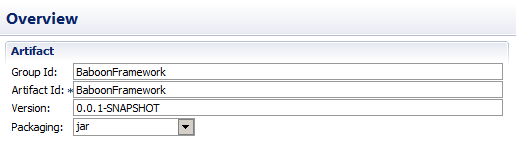
\includegraphics[width=80mm]{run_pom_file}
                \caption{Definición de Artefacto BaboonFramework en archivo
                pom.xml}
            \label{fig:run_pom_file}
                \end{figure}
          \item Abrir el archivo pom.xml del nuevo proyecto. Luego click en la
          pestaña “Dependencies”, en la parte inferior.
          \item Click en Add… y  luego completar los campos Group Id, Artifact
          Id y Version con los datos previos (Por ejemplo:
          BaboonFramework, BaboonFramework, 0.0.1-SNAPSHOT). Luego click en OK.
          \item Guardar el archivo pom.xml del proyecto.
          \item Click Derecho en el nuevo proyecto. Maven -\textgreater Update Project -\textgreater
          Ok
        \end{itemize}
\end{enumerate}


\subsection {Ejecución y Build del sistema utilizando \nombreFramework
Framework}

Para comenzar la ejecución del sistema desde la IDE Eclipse, debe seleccionarse
\emph{BaboonFramework} como punto de entrada al programa en las configuraciones:
    \begin{itemize}
      \item En Package Explorer, hacer click derecho sobre el proyecto.
      \item Seleccionar Run As -\textgreater Java Application.
      \item Seleccionar \emph{BaboonFramework}.
      \begin{figure}[H]
            \centering
            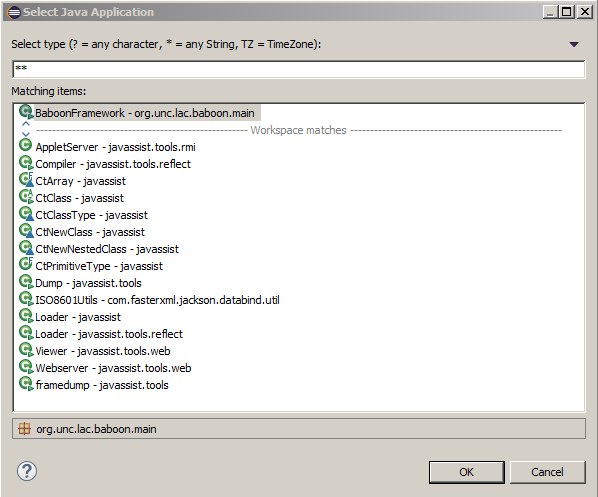
\includegraphics[width=90mm]{run_main_config}
            \caption{Clase Principal de un Sistema Desarrollado con Baboon Framework.}
            \label{fig:baboon_main}
      \end{figure}
    \end{itemize}

Para exportar un archivo JAR que ejecutable (requiere JRE \textgreater= 8) deben
realizarse los siguientes pasos:

\begin{enumerate}
  \item Incluir el archivo PNML y el archivo JSON de tópicos dentro de un
  paquete que forme parte del build path, como se observa en la
  figura~\ref{fig:run_recursos_topics_pnml}.
  \begin{figure}[H]
    \centering
    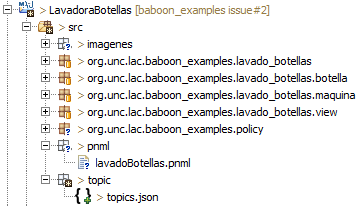
\includegraphics[width=70mm]{run_recursos_topics_pnml}
    \caption{Inclusión de Archivo PNML y Archivo de Tópicos en el Build
    Path}
    \label{fig:run_recursos_topics_pnml}
   \end{figure}
   En este caso, el path a los archivos debe especificarse en el programa de la
   siguiente forma:
   \begin{itemize}
     \item \textbf{\emph{``/topic/topics.json''}}
     \item \textbf{\emph{``/pnml/lavadoBotellas.pnml''}}
   \end{itemize}
   
   \item Dentro de las configuraciones del Build Path del proyecto, incluir
   las dependencias de Maven y las bibliotectas de AspectJ como exported
   entries, junto con el código fuente del framework, del monitor de RdP y del
   proyecto desarrollado:
    \begin{figure}[H]
    \centering
    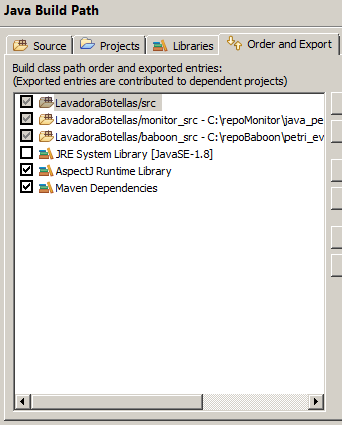
\includegraphics[width=60mm]{run_build_path}
    \caption{Configuración de Exported Entries en Build Path}
    \label{fig:run_build_path}
    \end{figure}
    
   \item Exportar un archivo JAR ejecutable.
       \begin{itemize}
         \item En Package Explorer, hacer click derecho sobre el proyecto.
         \item Seleccionar Export\ldots -\textgreater Runnable JAR File
         \item Elegir BaboonFramework como configuración de lanzamiento
         (esta configuración se hace visible una vez que se ha ejecutado
         el sistema utilizando \emph{Run As}, como se describe previamente).
         \item Elegir la opcion \emph{Extract required libraries into generated
         JAR} (Ver figura~\ref{fig:run_export_runnable_jar})
         \begin{figure}[H]
            \centering
            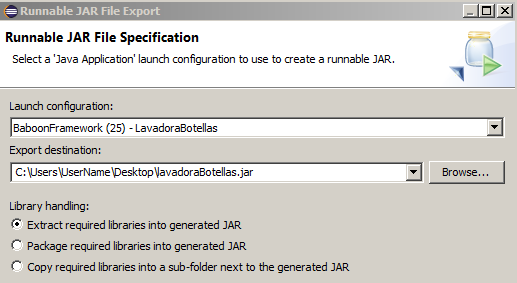
\includegraphics[width=70mm]{run_export_runnable_jar}
            \caption{Configuración de Archivo JAR Ejecutable}
            \label{fig:run_export_runnable_jar}
         \end{figure}
       \end{itemize}
\end{enumerate}